\chapter{From Theory to Practice: Applications and Interventions}
\label{chap7}

In the previous chapter, we uncovered that the Random Voting model can predict the scaled distributions of winner and runner-up vote across vastly different electoral units, from small polling booths to large parliamentary constituencies. This finding, alongside our earlier discovery of universal patterns in specific margin distributions, demonstrates how the Random Voting Model (RVM) can effectively predict electoral statistics across diverse contexts. These insights provide not just theoretical understanding but also practical tools for addressing real-world challenges in social systems.

This chapter explores two significant applications of our research: designing interventions to mitigate polarization in social networks and developing tools for detecting electoral malpractice. Both applications demonstrate how statistical physics principles can be applied to address societal challenges. We first examine how targeted interventions can reduce polarization in online discourse, then show how statistical patterns can help identify potential electoral irregularities. 

\section{Reducing Polarization in Social Networks}

Our research on opinion dynamics in Chapter 2 identified how polarized states emerge naturally in social systems, particularly in online networks where homophily—the tendency to interact with like-minded others—creates reinforcing echo chambers. The key insight from our modeling work is that these self-reinforcing patterns can be disrupted through carefully designed interventions.

\subsection{Challenges of Echo Chambers and Polarization}

Echo chambers represent a significant challenge to healthy discourse in modern digital environments. These self-reinforcing information environments arise through two primary mechanisms. First, homophily—our natural tendency to interact with like-minded others—creates initial clustering of similar opinions. Second, algorithmic recommendation systems on social platforms amplify this tendency by optimizing for engagement, often leading to content that reinforces existing beliefs rather than challenging them.

The consequences of these echo chambers extend to both individual and societal levels. Individuals exposed to increasingly homogeneous information tend to develop more extreme opinions and decreased tolerance for opposing viewpoints. At the societal level, this fragmentation undermines the shared factual basis necessary for productive public discourse and democratic decision-making. Our research in Chapter 2 demonstrated how these dynamics can be modeled mathematically, showing that polarized states emerge naturally from homophilic interactions even without external manipulation.

The challenge lies in developing interventions that can effectively disrupt these patterns without compromising user agency or platform viability. Any practical solution must balance the need to expose users to diverse viewpoints with respect for individual preferences and platform engagement metrics.

\subsection{The Random Nudge Intervention}

The ``random nudge" mechanism emerged as the most promising intervention strategy from our analysis. This approach introduces a controlled probability ($p$) that users encounter opinions outside their usual interaction patterns. When properly calibrated, this intervention reduces polarization while avoiding radicalization. Its implementation simplicity is valuable—requiring only a measured degree of randomness in recommendation algorithms without identifying users' specific political positions.

The intervention works by modifying the interaction probability between agents as:
\begin{equation}
    \widetilde{P}_{ij} = p \times \frac{1}{N-1} + (1-p) \times P_{ij}
\end{equation}
In this formulation, $\widetilde{P}_{ij}$ represents the modified interaction probability, $P_{ij}$ represents the original homophily-based interaction probability defined in Eq.~\ref{homophily.eq}, $N$ is the total number of agents, and $p$ is the nudge strength. Intuitively, this formula combines two components: a small random chance of interaction with any agent in the system, and the original preference-based interaction pattern. The parameter $p$ controls the balance between these components. This approach preserves most natural interaction patterns while introducing just enough randomness to prevent echo chamber formation.

In practice, this could be implemented by social media platforms as a subtle modification to their recommendation algorithms. For example, a platform might introduce a small probability that content from outside a user's typical interaction sphere appears in their feed. Importantly, this approach requires no knowledge of users' specific political positions—only the pattern of their past interactions—making it privacy-preserving and technically feasible.

\subsection{Practical Limitations and Considerations}

Despite its promise, the random nudge intervention faces several practical limitations. The primary challenge is calibration. Too little randomness fails to disrupt echo chambers, while excessive randomness risks pushing the system toward radicalization. Our optimization analysis showed that applying stronger interventions to a smaller subset of users often outperforms weaker interventions across the entire user base.

Platform incentives present another significant challenge. Social media companies optimize for engagement metrics that often benefit from the very echo chambers this intervention aims to disrupt. Implementing such changes would require either regulatory pressure or demonstrating that moderate depolarization can coexist with robust user engagement.

User resistance must also be considered. People naturally gravitate toward content that confirms their existing beliefs, and may disengage if exposed to too much challenging content. The intervention must be calibrated not just for mathematical optimality but also for psychological acceptability.

Finally, there are legitimate questions about who should determine the appropriate level of intervention. While our research provides mathematical guidance on optimal nudge strength, the decision to implement such systems ultimately involves value judgments about the proper balance between individual choice and collective discourse health.

\section{Safeguarding Electoral Integrity}

The universal patterns we discovered in electoral data offer not just theoretical insights but also practical tools for assessing election integrity. Our research identified two complementary approaches for detecting potential electoral malpractice: deviations from universality patterns and departures from Random Voting Model predictions.
\subsection{Electoral Malpractice: A Threat to Democratic Institutions}
Electoral malpractice undermines the foundational principle of democracy—that governance should reflect the genuine will of the people. When elections are manipulated, whether through ballot stuffing, voter intimidation, or administrative interference, this essential link between citizens and their government is broken. Beyond the immediate impact on specific election outcomes, persistent malpractice erodes public trust in democratic institutions and can lead to political instability, social unrest, and democratic backsliding.

The threat is particularly acute in emerging democracies where electoral systems may lack robust safeguards and independent oversight. However, even established democracies face challenges in maintaining electoral integrity, particularly as new technologies create both opportunities and vulnerabilities in electoral processes. The development of reliable methods for detecting potential malpractice is therefore crucial for protecting democratic governance worldwide.
\subsection{Challenges of Electoral Integrity Assessment}
Electoral integrity is fundamental to democratic governance, yet traditional methods for identifying malpractice often face significant limitations. Direct observation requires extensive resources and can only monitor a fraction of polling stations. Meanwhile, post-election surveys depend on respondents' willingness to accurately report experiences, which may be compromised in environments where intimidation is present.

Statistical approaches offer a complementary tool that can identify patterns of irregularity across entire electoral systems. Previous work by Klimek et al. \cite{klimek2012statistical} and Jiménez et al. \cite{jimenez2017testing} has explored using statistical indicators to detect potential fraud. Our research extends these toolkit by providing a robust, theoretically grounded framework based on universal statistical patterns observed across diverse electoral contexts.
\subsection{Flagging Potential Electoral Malpractice}
Our analysis revealed pronounced deviations from the universal pattern in certain electoral contexts. Figure \ref{fig:malpractice} shows how the distributions for Ethiopia (2010) and Belarus (2004-2019) diverge significantly from the expected pattern predicted by the Random Voting Model as well as the universal distribution of scaled specific margin.
\begin{figure}[h]
    \centering
    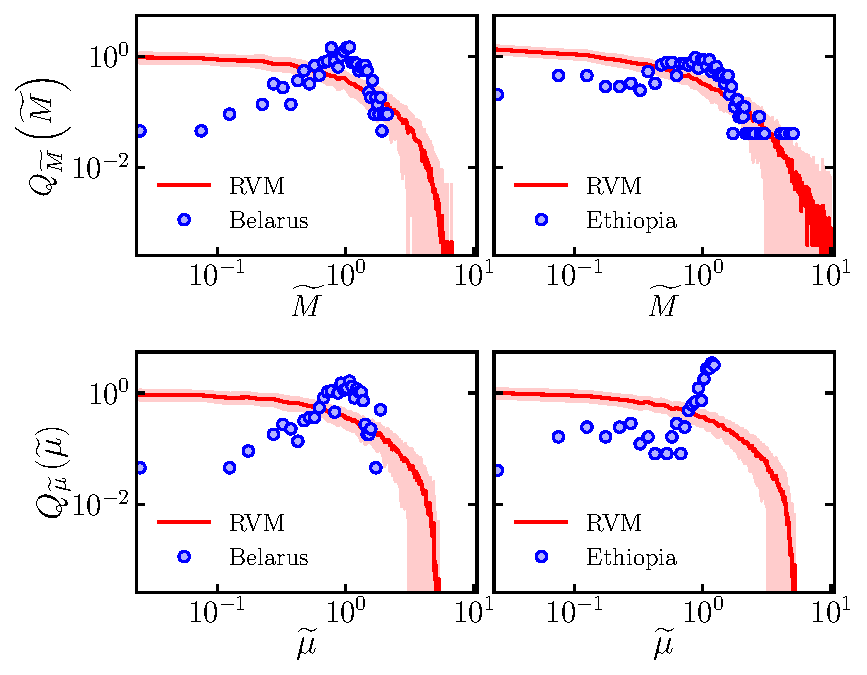
\includegraphics[width=\textwidth]{chapters/chapter7/malpractice_flag.pdf}
    \caption{Detecting electoral malpractice through statistical signatures. The distributions (a) $Q_{\widetilde{M}}(\widetilde{M})$, and (b) $Q_{\widetilde{\mu}}(\widetilde{\mu})$ obtained from empirical data from Belarus $(2004-2019)$ and Ethiopia $(2010)$ (blue circles) show significant deviation from the model predictions (red line). The light red shaded region represents the variability in RVM prediction computed from 100 realizations. These deviations from expected patterns suggest potential electoral irregularities that warrant further investigation.}
    \label{fig:malpractice}
\end{figure}
In both cases, the distributions show an overrepresentation of large margins and specific margins compared to what would be expected in competitive electoral environments. This pattern is consistent with reports from independent electoral observers who documented concerns about these elections.

Our framework provides two complementary tools for flagging potential electoral malpractice. First, deviations from universality: The scaled distribution of margin-to-turnout ratio should follow a universal form across all competitive elections. Significant departures from this universal pattern can indicate manipulation. Second, departures from Random Voting Model predictions: The RVM accurately predicts scaled margin distributions across diverse electoral contexts when using actual turnout data as input. When empirical margin distributions deviate substantially from these predictions, this suggests non-random influences on voting patterns.

These statistical methods offer several advantages over traditional monitoring approaches. They can be applied retrospectively to historical data, allowing for the identification of patterns that might have been missed during the election. They also provide a quantitative baseline against which to compare future elections, potentially signaling deterioration or improvement in electoral integrity over time. Most importantly, they can analyze entire electoral systems rather than samples, potentially revealing systemic patterns of irregularity that might be missed by more localized approaches.

\subsection{Implementation Challenges and Limitations}

While our statistical approach offers powerful tools for identifying potential electoral malpractice, several important caveats must be considered in practical implementation. 

Statistical signatures cannot definitively prove malpractice alone—they identify patterns warranting further investigation and should complement other forms of evidence including observer reports and historical context. 

Not all deviations necessarily indicate fraud; legitimate factors like unusual demographics or natural disasters can cause statistical anomalies. These methods work best with sufficient data points, making them most reliable for elections with numerous electoral units. 

Ultimately, detection is only the first step—effective remediation requires robust legal frameworks, independent electoral commissions, and political will to enforce consequences for violations.
\section{Summary and Outlook}
In this chapter, we have demonstrated how the theoretical insights developed throughout this thesis can be translated into practical applications. From designing interventions to mitigate polarization in social networks to developing statistical methods for detecting electoral malpractice, our research offers tools to address significant societal challenges.

The random nudge intervention provides a promising approach for reducing polarization without compromising user privacy or engagement. By introducing controlled randomness into user interactions, this mechanism can effectively break echo chambers while avoiding the risks of radicalization.

Similarly, our statistical framework for detecting electoral malpractice offers a useful complement to traditional monitoring approaches. By identifying deviations from universal patterns and Random Voting Model predictions, this framework can help safeguard democratic processes and strengthen electoral integrity.

Both applications highlight the value of statistical physics approaches to social phenomena. By identifying underlying universal patterns and developing models that capture essential dynamics, we can gain insights that transcend specific contexts and inform effective interventions.

The final chapter will synthesize these findings, discuss limitations of our current approaches, and outline directions for future research that could further enhance our understanding of social systems and their practical applications.